\subsection{Workflow Abstraction using Motifs}
\label{sec:abstraction}
%Depending on the context of the deliverable, this first paragraph may be commented. 
%Scientific workflows have been increasingly used in the last decade as an instrument for data intensive science. 
Workflows serve a dual function: first, as detailed documentation of the scientific method used for an experiment (i. e. the input sources and processing steps taken for the derivation of a certain data item), and second, as re-usable, executable artifacts for data-intensive analysis. 
Scientific workflows are composed of a variety of data manipulation activities such as Data Movement, Data Transformation, Data Analysis and Data Visualization to serve the goals of the scientific study. The composition is done through the constructs made available by the workflow system used, and is largely shaped by the function undertaken by the workflow and the environment in which the system operates.

A major difficulty in understanding workflows is their complex nature. A workflow may contain several scientifically significant analysis steps, combined with other Data Preparation or result delivery activities, and in different implementation styles depending on the environment and context in which the workflow is executed. This difficulty in understanding stands in the way of reusing workflows.

As a first step towards addressing this issue \cite{garijo_Alper_2012} describes a catalogue of domain independent conceptual abstractions for workflow steps called scientific Workflow Motifs. The catalogue was built based on an empirical analysis performed over 260 workflow descriptions from Taverna \cite{taverna}, Wings \cite{DBLP:journals/expert/GilRKGGMD11}, Galaxy \cite{Goecks_Nekrutenko_Taylor_2010} and Vistrails \cite{Callahan06-vistrails}. Motifs are provided through i) a characterization of the kinds of data-oriented activities that are carried out within workflows, which are referred to as Data-Operation motifs, and ii) a characterization of the different manners in which those activity motifs are realized/implemented within workflows, referred to as Workflow-Oriented motifs. Figure \ref{fig:tav_wf_motifs} shows an example of a Taverna workflow with its motifs highlighted. The workflow transfers data files containing proteomics data to a remote server and  augments several parameters for the invocation request. Then the workflow waits for job completion and inquires about the state of the submitted warping job. Once the inquiry call is returned the results are downloaded from the remote server.

\begin{figure*}[ht!]
\centering
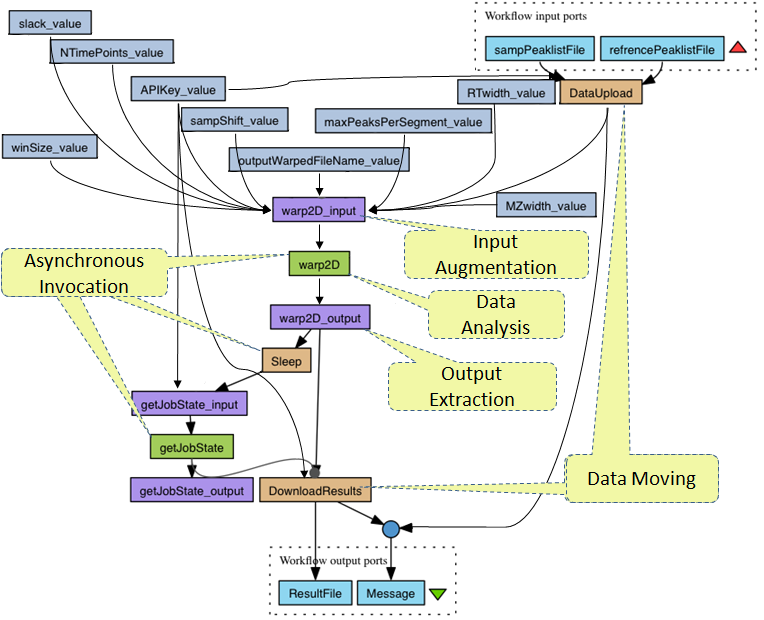
\includegraphics[scale=0.70]{Figures/taverna-wf-motifs.png}
\caption{\textcolor{black}{Sample motifs in a Taverna workflow for functional genomics.}}
\label{fig:tav_wf_motifs}
\end{figure*}

This section describes the Workflow Motifs ontology\footnote{http://purl.org/net/wf-motifs}, an OWL 2 encoding ot the aforementioned motif catalogue. The goal of this ontology is to provide the means to annotate workflows and their steps with the motifs of the vocabulary, without setting any restriction on how the workflows are defined themselves.

\subsubsection{Representing Motifs}
Figure \ref{fig:ontology} shows an overview of the class taxonomy of the ontology. The class {\tt  Motif} represents the different classes of motifs identified in the catalog. This class is categorized into two specialized sub-classes {\tt  DataOperationMotif} and {\tt  WorkflowMotif}, which are sub-classed following the taxonomy represented in \cite{garijo_Alper_2012}.

\begin{figure*}[t!]
\centering
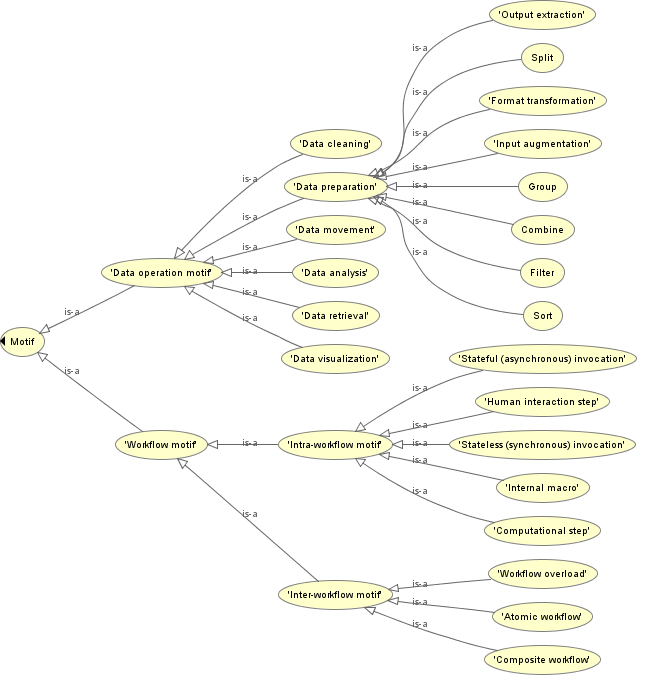
\includegraphics[scale=0.60]{Figures/ontology.png}
\caption{\textcolor{black}{Diagram showing an overview of the class taxonomy of the motif OWL ontology.}}
\label{fig:ontology}
\end{figure*}  

The ontology provides three properties to link motifs to workflow specifications and their fragments. The {\tt  hasMotif} property associates workflows and their operations with their motifs. The properties {\tt  hasDataOperationMotif} and {\tt  hasWorkflowMotif} allow annotating workflows and their steps with more specificity. These properties have no domain specified, as different workflow models may use different vocabularies for describing workflows and their parts. 

\subsubsection{Representing Workflows and Workflow Steps}
Workflows may be represented with different models and vocabularies like OPMW \cite{garijo_gil_2011}, P-Plan  \cite{garijo-gil-lisc12} or D-PROV \cite{Missier2013a}. While providing an abstract and consistent representation of the workflow is not a pre-requisite to the usage of the Motif ontology, we consider it a best-practice to use a model that is independent from any specific workflow language or technology. An example of annotation using the wfdesc model is given in Figure \ref{fig:annot-example} by showing the annotations of part of the Taverna workflow shown in Figure \ref{fig:tav_wf_motifs}. 

\begin{figure*}[ht!]
\centering
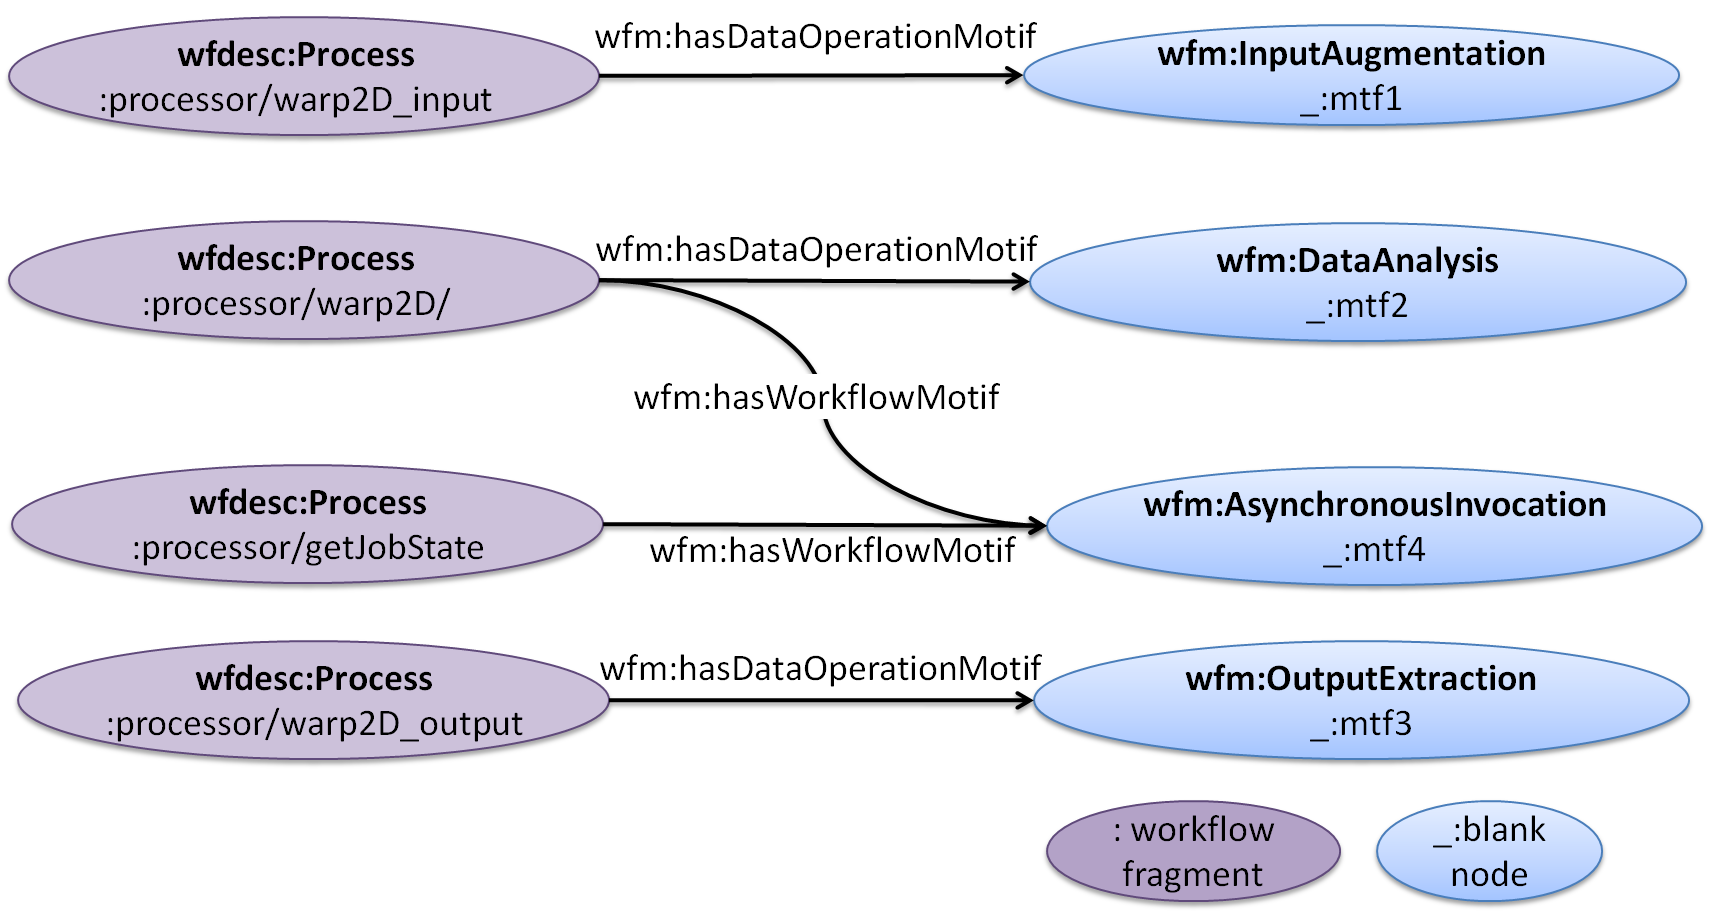
\includegraphics[scale=0.2]{Figures/tav-wf-annotated.png}
\caption{Subset of the annotations of the Taverna workflow shown in Figure \ref{fig:tav_wf_motifs} using the wfdesc model.}
\label{fig:annot-example}
\end{figure*} 

The annotations encoded using the Motif Ontology could be used in a variety of applications. By providing explicit semantics on the data processing characteristic and the implementation characteristic of the operations, annotations improve understandability and interpretation. Moreover, they can be used to facilitate workflow discovery. For example, the user can issue a query to identify workflows that implement a specific flow of data manipulation and transformation (e.g., {\em return the workflows in which data reformatting is followed by data filtering and then data visualization}). Having information on characteristics of workflow operations allow for manipulation of workflows to generate summaries \cite{summaryBigData13} of workflow descriptions or their execution traces.
 
